\chapter{Spectroscopic Sky Surveys}
\label{data_chapter}

% TODO chapter introduction

Select suitable dataset of astronomical spectra for experiments.

To understand this work we need first to introduce the spectral
data because we are interested in classifying them.

\section{Astronomical Spectroscopy}

Almost all we know about the universe outside our solar system
is based on the analysis of ligth, i.e. \textit{electromagnetic} (EM) radiation
by observing its flux, time variations, etc.~\cite{appenzeller2012}
Spectroscopy started when Issac Newton carried out the experiment of light decomposition throgh a prism in 1666.
Next, Thomas Young has shown that light behaves like a wave.
However, EM radiation exhibits also particle nature.

The particles of EM radiation are photons.
Photons has no mass but transport energy and have momentum.
Every photon has an associated frequency \(\nu\)
of the corresponding EM wave giving it a energy
by the Planck--Einstein relation:

\begin{equation}
	E = h \nu,
	\label{planck_einstein_equation}
\end{equation}

where \(h\) is the Planck constant and \(\nu\) is frequency of the photon.
Therefore, higher frequency means higher energy.
All photons in vacuum move in the speed of light \(c\).
The frequency \(\nu\) is related to the wavelength \(\lambda\):

\begin{equation}
	\nu = \frac{c}{\lambda},
	\label{frequency_wavelength_equation}
\end{equation}

where \(c\) is the speed of light.
Combining equations~\ref{planck_einstein_equation} and \ref{frequency_wavelength_equation} gives:

\begin{equation}
	E = h \frac{c}{\lambda}.
	\label{energy_wavelength}
\end{equation}

We see that energy of a photon is inversly proportional to wavelength \(\lambda\).~\cite{trypsteen2017}

Secondly, EM radiation has the wave nature. 
EM wave also propagetes in the speed of light \(c\) and transfers energy.
Again the higher the frequency the more energy it carries.~\cite{cochard2018}

EM wave can be decomposed (by a prism or a diffraction grating)
as a function of its wavelength \(\lambda\).
The complete decomposed spectrum of EM radiation is called the EM spectrum.
The visible light is only a tiny part of the complete spectrum of electromagnetic radiation.
The complete spectrum consists of \(\gamma\)~rays, X-rays, ultraviolet, visible light, infrared radiation, microwaves, radio waves (see Table~\ref{em_spectrum}).

\begin{table}
\begin{center}
\begin{tabular}{|l|r|}
	\hline
	Radiation type & Wavelength (m) \\ \hline \hline
	\(\gamma\) ray & \(10^{-12}\) \\ \hline
	X-ray & \(10^{-10}\) \\ \hline
	Ultraviolet & \(10^{-8}\) \\ \hline
	Visible & \(0.5 \times 10^{-6}\) \\ \hline
	Infrared & \(10^{-5}\) \\ \hline
	Microwave & \(10^{-2}\) \\ \hline
	Radio & \(10^{3}\) \\ \hline
\end{tabular}
\end{center}
\caption{Parts of electromagnetic spectrum}
\label{em_spectrum}
\end{table}

EM radiation is produced by either heating up matter or by exciting atoms.
The blackbody is a physical model of spectral radiation \(B(\lambda, T)\).
Max Planck derived the spectral distributon of a black body.
Heating transforms into an emission of EM radiation at all wavelengths
with an energy distribution as a function of wavelength
which only depends on the temperature and is described by Planck's law:

\begin{equation}
	B(\lambda, T) = \frac{2 h c^2}{\lambda^5}
	\frac{1}{e^{\frac{hc}{\lambda k_{\mathrm{B}}T}} - 1}
\end{equation}

where \(k_{\mathrm{B}}\) is the Boltzmann constant 
and \(h\) is the Planck constant.
This phenomenon does not depend on the composition of the body
but only on its temperature.
The Wien's displacement law gives the wavelength of maximum intensity \(\lambda_{\max}\):

\begin{equation}
	\lambda_{\max} = \frac{b}{T}
\end{equation}

where \(b\) is the Wien's displacement constant.
Accordingly, we can derive the temperature \(T\) of an object
with known wavelength of maximum intesity \(\lambda_{\max}\):

\begin{equation}
	T = \frac{b}{\lambda_{\max}}.
\end{equation}

where \(b\) is the Wien's displacement constant.~\cite{cochard2018}

We consider stars to be black bodies
because they are objects hotter than its environmenti
and emit electromagnetic radiation.
Therefore, all EM radiation of a star is determined only by its temperature.
The other way around, with the Wien's displacement law
we can estimate the absolute temperature \(T\) of a star.~\cite{trypsteen2017}

The undisturbed profile of a continuum level \(I(\lambda)\)
represents roughly the temperature dependence on
blackbody radiation characteristics \(B(\lambda, T)\).

% TODO show image continuum

Secondly, EM radiation can be emitted by exciting atoms.
Therefore, EM radiation carries information about stars and planets
made of matter across the universe.
The energy carried by EM radiation interacts with matter in following ways:

\begin{itemize}
	\item \textit{emission} occurs when EM radiation propages throught a gas
		because the atoms of the gas might exite ane emit EM radiation;
	\item \textit{absorption} happens when a gas absorbs some wavelengths
		of the EM radiation.
\end{itemize}

Fraunhofer was also one of the first to observe dark lines in the solar spectrum
and David Brewster postulated that the dark lines correspond to absoption from gas in the way of light travelling towards us.
Robert Wilhelm Bunsen and Gustav Kichhoff showed that each chemical element has its own set of spectral lines
and Kichhoff established the three famous laws describing the three types of spectra:

\begin{itemize}
	\item the spectrum of a conventional light bulb is a continuous rainbow (called \textit{continuos spectrum});
	\item if a cloud of gas lies between a detector and a bulb,
		the cloud can absorb specific wavelength making what an \textit{absorption-line spectrum};
	\item if a cloud emits light itself its spectrum is called an \textit{emission-line spectrum}.
\end{itemize}

Real astronomical spectra are usually a combination of these types.
Therefore, spectrocopy can be used for chemical analysis of matter.
Then, at the beginning of the twentieth century,
the invention quantum mechanics help us to understand the origin of spectral lines.

We model matter as made of atoms.
An atom has a specific number of electrons
which are place in particular orbits of the atom.
Electrons in an orbit have a specic energy level.
We know from quantum mechanics that an electron can change energy level by an exchange of energy in form of a photon.
The energy transfer is not continuous.
The energy has to precisily correspond to the difference in the energy levels.
Therefore the change produces a EM radation with an energy \(E\) in the wavelength \(\lambda\)
according to Planck--Einstein relation~\ref{energy_wavelength}.
Therefore, the specific set of energy levels of a atom detemines
if photons are either absorped or emitted by it.
This is a direct consequence for spectroscopy.~\cite{cochard2018}

The fact that each atom,
ion or molecule possesses a unique set of energy levels
causes emission and absorption lines at specific wavelengths in spectra.
Spectral lines correspond to the wavelengths of light absorbed by chemicals on the surface of the star.
Therefore, positions of emission and absorption lines can tell us objects composition.
We display spectra as bands of light that is a projection of light
that passes through a prism on a wall (see Fig.~\ref{solar_spectrum})
called \textit{two-dimensional} spectra.~\cite{cochard2018}

\begin{figure}
% source https://solarsystem.nasa.gov/resources/390/the-solar-spectrum/
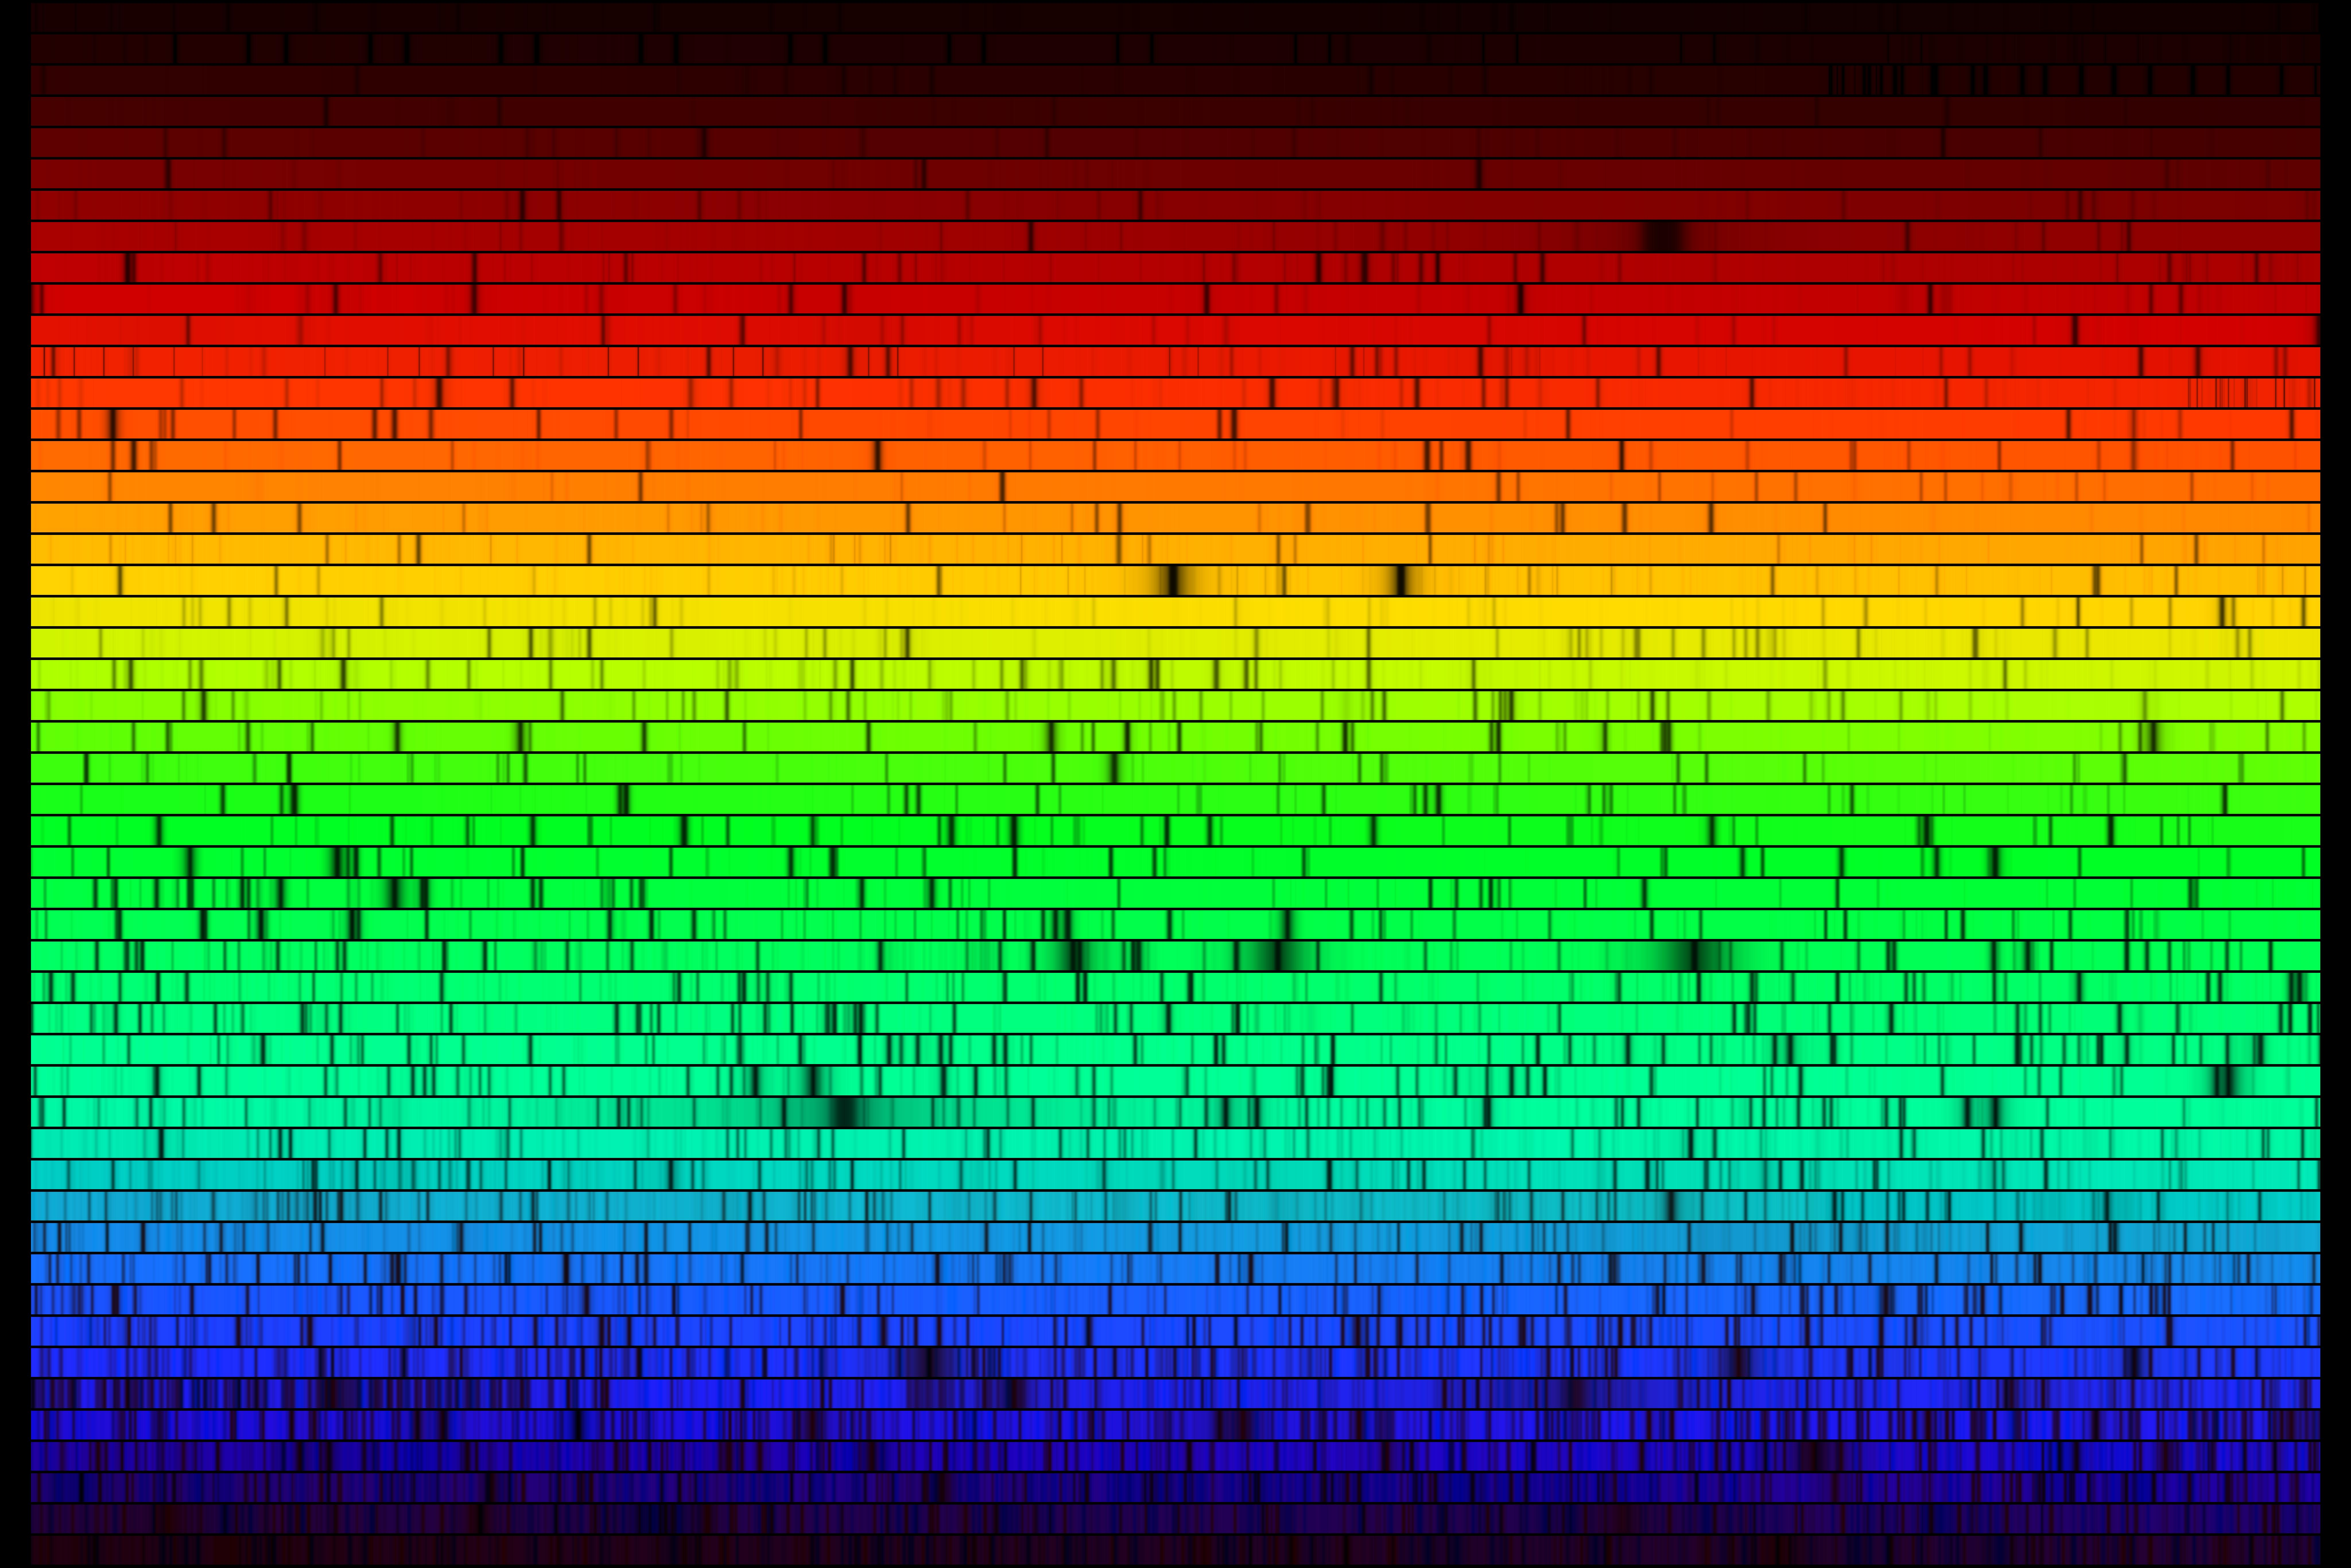
\includegraphics[width=\textwidth]{img/solarspectrum.jpg}
\caption[The Solar spectrum]{
	The specturm of the Sun. (Image by \href{https://solarsystem.nasa.gov/resources/390/the-solar-spectrum/}{NASA}.)
}
\label{solar_spectrum}
\end{figure}

A more reasonable way is to display spectra as graphs of intensities of the light as the vertical axis and wavelengths as the horizontal axis:
called a \textit{one-dimensional spectral profile}.~\cite{cochard2018}
This representation of a astronomical spectrum can be seen as a one-dimensional image.~\cite{bennett2005}

% TODO one-dimensional spectrum

% TODO Christian Doppler discoverd the Doppler effect that allowed to measure the motion of celestial objects using Doppler shift in its spectrum.

Joseph von Fraunhofer was the first to observe spectra of stars by using spectroscope in combination with telescope.
Nowadays, new technologies have advanced spectroscopic observations
(CCD detectors, optical fibers and computing power).~\cite{cochard2018}
Telescopes are giant eyes that can collect much more light that an eye of a human.
A telescope is composed of mirror that lead light into a spectrograph.
A spectrograph contains a diffraction grating and a \textit{charge-coupled device} (CCD) camera.
Diffration grating was invented by Fraunhofer based on the wave nature of light.
Diffration grating can disperse the light collected by a telescope into a spectra
while allowing greater dispersion than prisms.
on gratings are one of the essential parts of modern spectroscopes
Then the dispersed specturm reveals objects composition, speed, temperature
and more.~\cite{bennett2005}

Photons carry information about observed objects
to a pixel of a CCD camera in a telescope.
CCD cameras require the particle nature of light (electromagnetic radiation).~\cite{trypsteen2017}

The most important parameters of a telescope are
\textit{resolving power}, \textit{signal-to-noise ration}
and \textit{signal-to-noise ration}.

Resolving power \(R\) experess capacity of a telescope to oberve details of a spectrum.
Resolving power is defined as:

\begin{equation}
	R = \frac{\lambda}{\Delta \lambda}
\end{equation}

where \(\lambda\) is considered wavelength
and \(\Delta \lambda\) is the smallest visible detail.

% TODO is it a parameter of a telescope or spectrum?
\textit{Signal-to-noise ratio} (SNR) is a parameter of our instrument.
We can trust our measurment when signal is high in compared to nise.~\cite{cochard2018}

\textit{Full width at half maximum} (FWHM) is the measurement of the width of a spectral line
at the half of its maximum intensity measured from the continuum.
FWHM is determined by the width of a slit which makes the broadening of a line.
A perfect instrument would have an infinitely thin line.

\section{Quasi-Stellar Objects}

Quasi-stellar (star-like) objects (also known as \textit{quasars} and abbreviated \textit{QSO}) are the most luminious \textit{active galactic nuclei} (AGNs).~\cite{beckmann2013}

The physical model is a supermassive black hole surrounded by a gaseous accretion disk.
A QSO generates energy by stress and friction in the disk outside ot the black hole because no light can escape the \textit{event horizont}.
The energy is in form of electromagnetic radiation and is the strongest in the ultraviolet band.
Moreover, QSOs exhibit big cosmological redshift.

QSOs were common in the early universe probably because galaxies have run out of matter: they stop to be so lumionious.
Therefore, QSOs help us to study the early universe.

There are different types of QSOs: radio-loud, radio-quiet, broad absorption-line, type II, red, optically violent variable, weak emission-line.

\begin{itemize}
	\item Physical definition of QSOs.
	\item Definition of QSOs according SDSS DR14Q.
	\item Why QSOs are suitable for experimenting with DA?
		QSOs have big redshift and CNNs are shift invariant.
		Searching for QSOs in different archives.
\end{itemize}

\begin{figure}
\begin{center}
\subfloat[Best image of bright quasar 3C 273][
	Best image of the bright quasar 3C 273
	(Image by \href{https://www.spacetelescope.org/images/potw1346a/}{ESA/Hubble} is licensed under CC BY 4.0)
	]{
	% TODO give credit https://www.spacetelescope.org/images/potw1346a/
	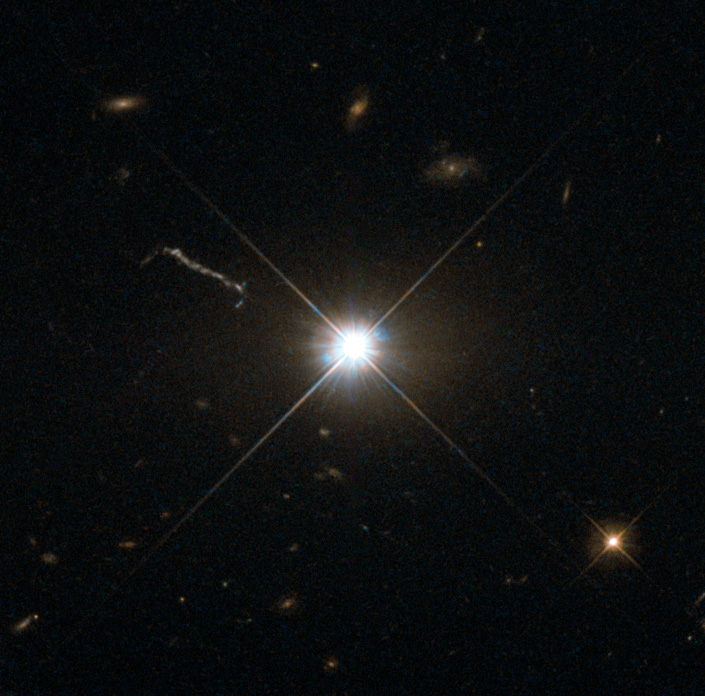
\includegraphics[height=0.45\textwidth]{img/potw1346a.jpg}
	}
\subfloat[Jet]{
	% TODO give credit https://chandra.harvard.edu/photo/2000/0131/index.html
	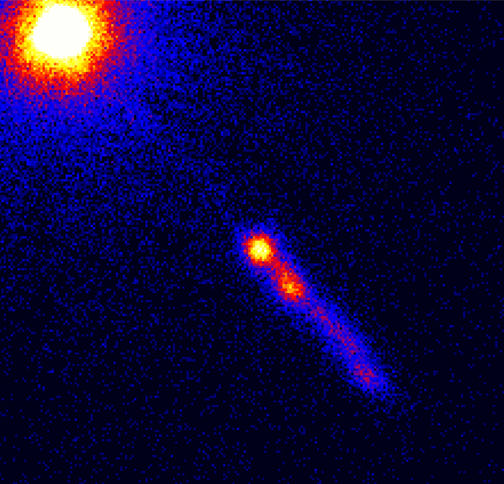
\includegraphics[height=0.45\textwidth]{img/0131_xray.jpg}
	}
\end{center}
\caption{
The first ever discover quasar 3C 273.
}
\label{3c_273}
\end{figure}

\begin{figure}
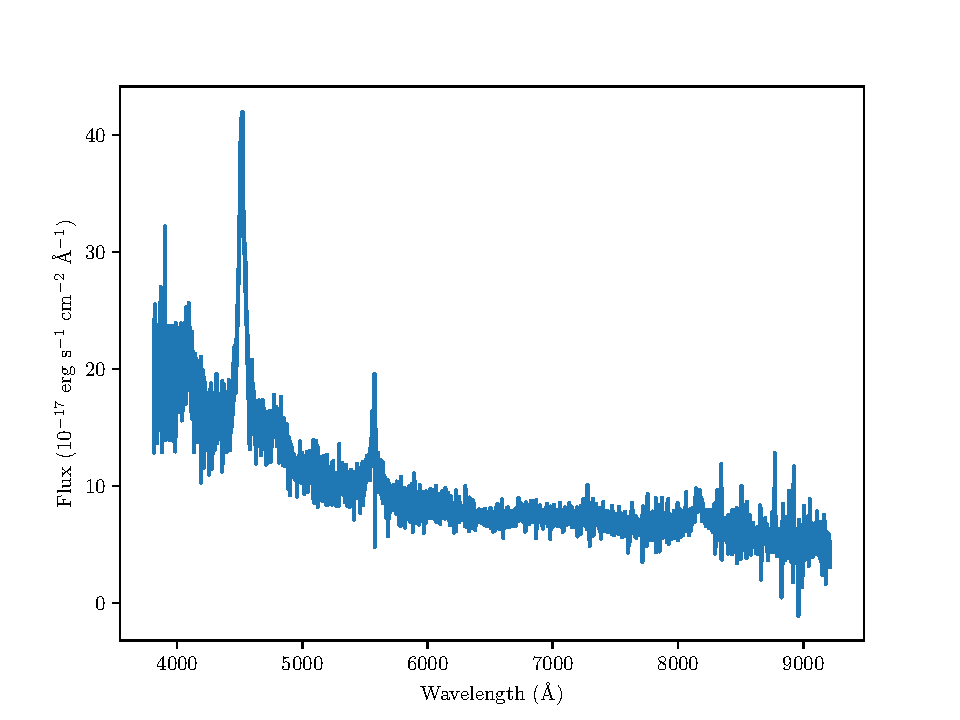
\includegraphics[width=\textwidth]{img/spec_3c_273.pdf}
\caption{Spectrum of the QSO 3C 273}
\label{3c_273_spectrum}
\end{figure}

\section{Large Spectroscopic Surveys}
\label{large_spec_surveys}

Since the discovery of first QSO,
there has been a huge progress in spectroscopy allowing observing
vast amount of spectra and QSOs.
It started with Bright Quasar Survey, Large Bright Quasar Survey (LBQS)
and 2dF Quasar Redshift Survey.
Their big successors are the \textit{Sloan Digital Sky Survey} (SDSS)
and the \textit{Large Sky Area Multi-Object Fiber Spectroscopic Telescope} (LAMOST)
that already contain millions of spectra.
We choose LAMOST and SDSS surveys for our experiments
because they offer large volume of data suitable for machine learning
and training neural networks for domain adaptation.

In the two following subsections,
we introduce the paramaters of their instruments,
their recent data releases and corresponding catalogs of QSOs.

\subsection{Sloan Digital Sky Survey}
\label{sdss}

SDSS is in opeation since 2000
and its telescope is designed to provide both a photometrically
and astrometrically calibrated imaging survey
and a spectroscopic survey of galaxies and QSOs.~\cite{york2000}

The SDSS survey uses a 2.5~m telescope located at the Apache Point Observatory, New Mexico (see~Figure~\ref{sdss_telescope}).
The telescope has 3\(^{\circ}\) fild of view due to the mirror.
The original spectrograph of the telescope was able to obtain 640 spectra
with a wavelength coverage 380--920~nm simultaneously
with spectral resolution \(R \sim 1\,800\).~\cite{gunn1998, york2000}

\begin{figure}
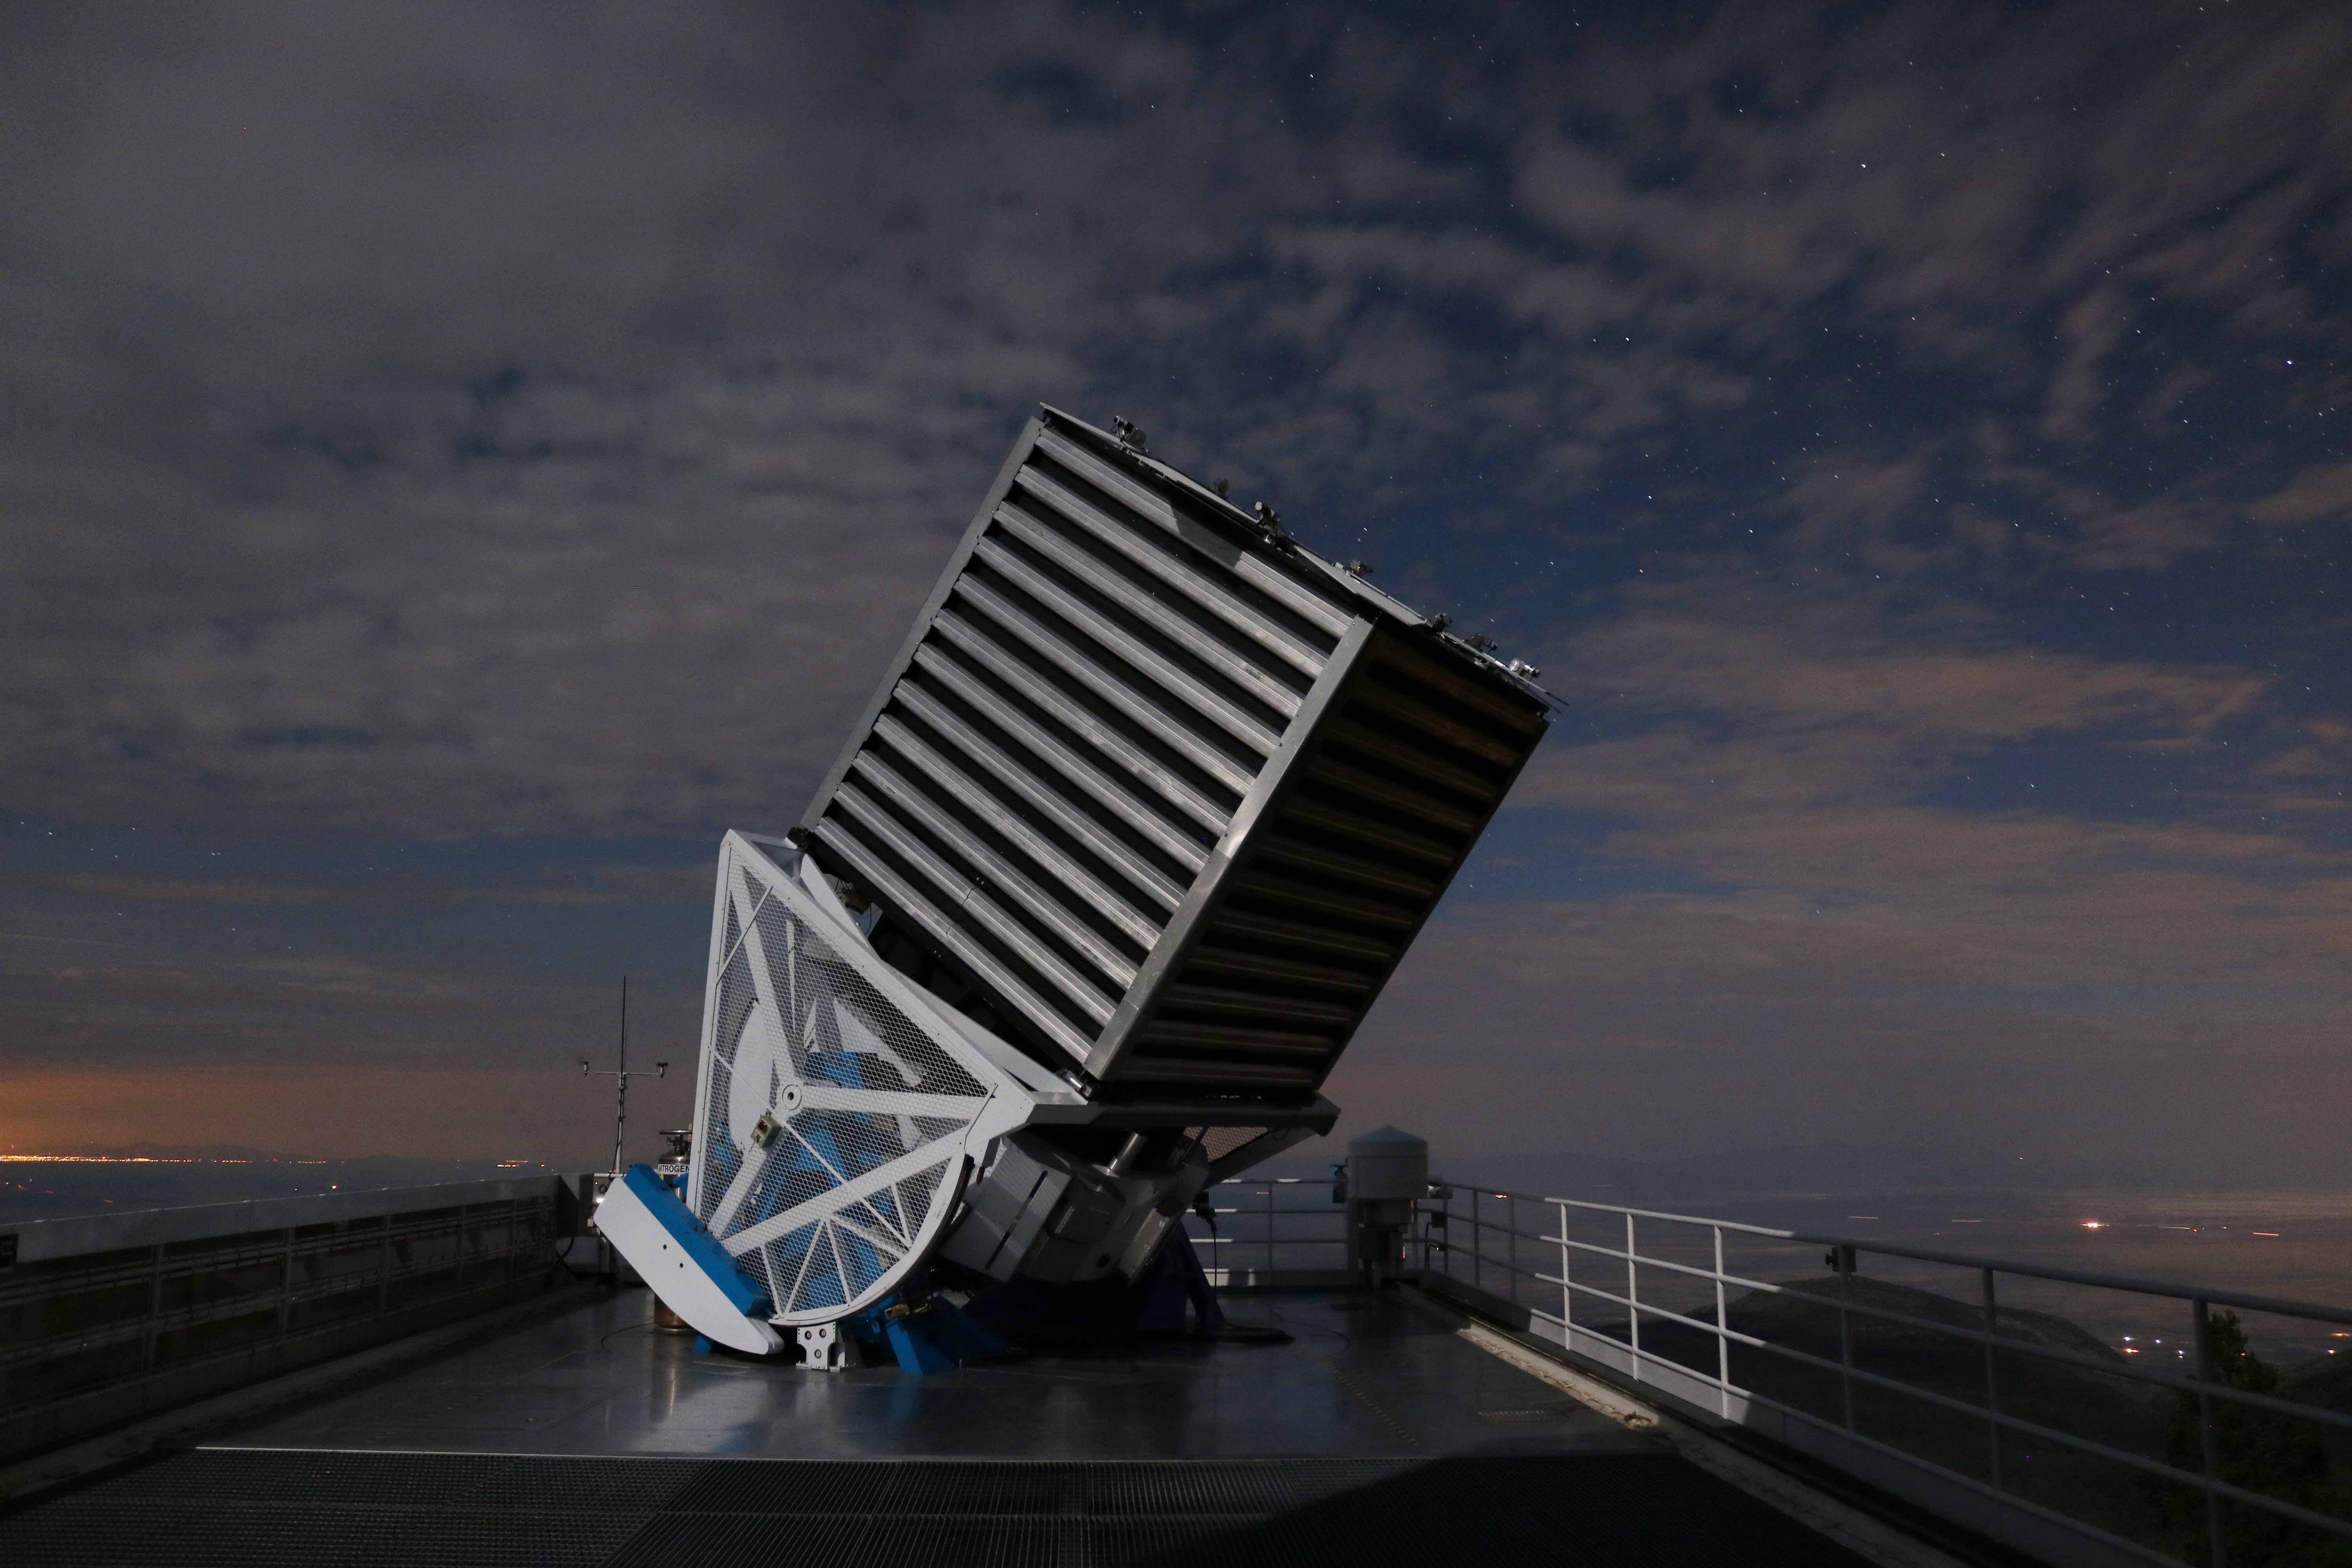
\includegraphics[width=\textwidth]{img/sdss_gaulme.jpg}
\caption[The SDSS telescope]{
	The SDSS telescope at night.
	(Image by Patrick Gaulme is licensed under CC BY 4.0.)
	}
\label{sdss_telescope}
\end{figure}

In 2009, the original spectrograph was upgraded for \textit{Baryon Oscillation Spectroscopic Survey} (BOSS).
The upgraded BOSS spectrograph covers a wavelength range 356--1\,040~nm
with resolving power \(R \sim 2\,000\)
and is capable to 1\,000 spectra at once.~\cite{smee2013}

Its recent SDSS Data Release 14 (SDSS DR14) which corresponds to the latest catalog of QSOs
contains more than one-third of the entire celestial sphere.
The total number of optical spectra is 4\,851\,200.

The SDSS Data Release 14 Quasar (SDSS DR14Q) catalog described in~\cite{paris2018}.
The SDSS DR14Q catalog contains 526\,356 quasars (contamination is estimated to be about 0.5\%).
SDSS provides calibrated spectra covering the wavelength range 3\,610--10\,140~\AA{} at a spectral resolution 1\,300 < \(R\) < 2\,500 for all the quasars.

% TODO define luminosity
The catalog defines a quasar is an object with a luminosity \(M_i[z = 2] < -20.5\)
and either displaying at least one emission line with FWHM > 500~km~s\(^{-1}\) or,
if not, having interesting absorption features.

\subsection{Large Sky Area Multi-Object Fiber Spectroscopic Telescope}
\label{lamost}

LAMOST survey was launched in 2012
and has two primary scientific goals to explore both extragalactic
and intragalactic phenomenons.
Therefore, unlike SDSS LAMOST also observes large volume of stars.
However, the other scientific goal of LAMOST is the extragalactic spectroscopic survey of the large scale structure of the universe and the physics of galaxies.
The goal includes spectroscopic survey of nearly 10 millions galaxies and \textit{quasars}
that will contribute to the study of the accretion process of massive black holes in AGNs besides other things.~\cite{cui2012}

The LAMOST is located in Xinglong Station of national Astronomical Observatory, China.
The telescope is a special telescope with a primary mirror made of 37 hexagonal spherical mirros of total size 6.67~m times 6.05~m.
The large primary mirror makes the field of view of 5\(^{\circ}\).
The focal surface has 4\,000 fibers connected to 16 spectrographs with 32 CCD cameras.
Therefore, the telescope is capable of observing up to 4\,000 spectra simultaneously
in a wavelength coverage of 370--900~nm with spectral resolution \(R = 1\,000\) or \(R = 1\,500\) depending on gratings and camera positions.~\cite{cui2012}

LAMOST Data Release 5 v3 (LAMOST DR5) released in June 2019
contains 9\,026\,365 optical spectra.
LAMOST released three catalogs of QSOs
(DR1~\cite{ai2016}, DR2\&3~\cite{dong2018} and DR4\&5~\cite{yao2019})
that in total contains 42\,552 spectra of QSOs.

\subsection{Comparison of the Spectral Data}

Now, we compare the SDSS and LAMOST survey
to prove their suitability for domain adapation.
The surveys are mainly different in term of instruments, sky coverage and target strategy.

Concerning the instrument we summarise the main parameters of telescopes
of the surveys in Table~\ref{telescopes_parameters}.
We see that LAMOST has lower resolution and shorter wavelength coverage than SDSS.
However, SDSS has smaller field of view.

\begin{table}
\begin{center}
\begin{tabular}{|l|r|r|r|}
	\hline
	Parameter of a telescope & SDSS & BOSS & LAMOST \\
	\hline \hline
	wavelength coverage (nm) & 380--920 & 356--1\,040 & 370--900 \\ \hline
	spectral resolution \(R\) & 1\,800 & 2\,000 & 1\,250 \\ \hline
	field of view & \multicolumn{2}{|c|}{3\(^{\circ}\)} & 5\(^{\circ}\) \\ \hline
\end{tabular}
\end{center}
\caption{Parameters of telescopes}
\label{telescopes_parameters}
\end{table}

Sky coverage is very connected to the targeting strategy or scientific goals.
Figure~\ref{sky_coverage} displays sky coverage of both SDSS and LAMOST.
We see that SDSS does not observe our Milky Way galaxy.
On the other hand LAMOST observes everywhere on the notrh hemisphere
but is not able to obserce close to zenit due to its construction limits.

From the perspective of coverage of QSOs depicted in Figure~\ref{qso_coverage}
LAMOST did not observe QSOs in some part of sky
where QSOs are abundant according to SDSS.

% TODO 90 is not complete in charts
\begin{figure}
\begin{center}
\subfloat[][]{
	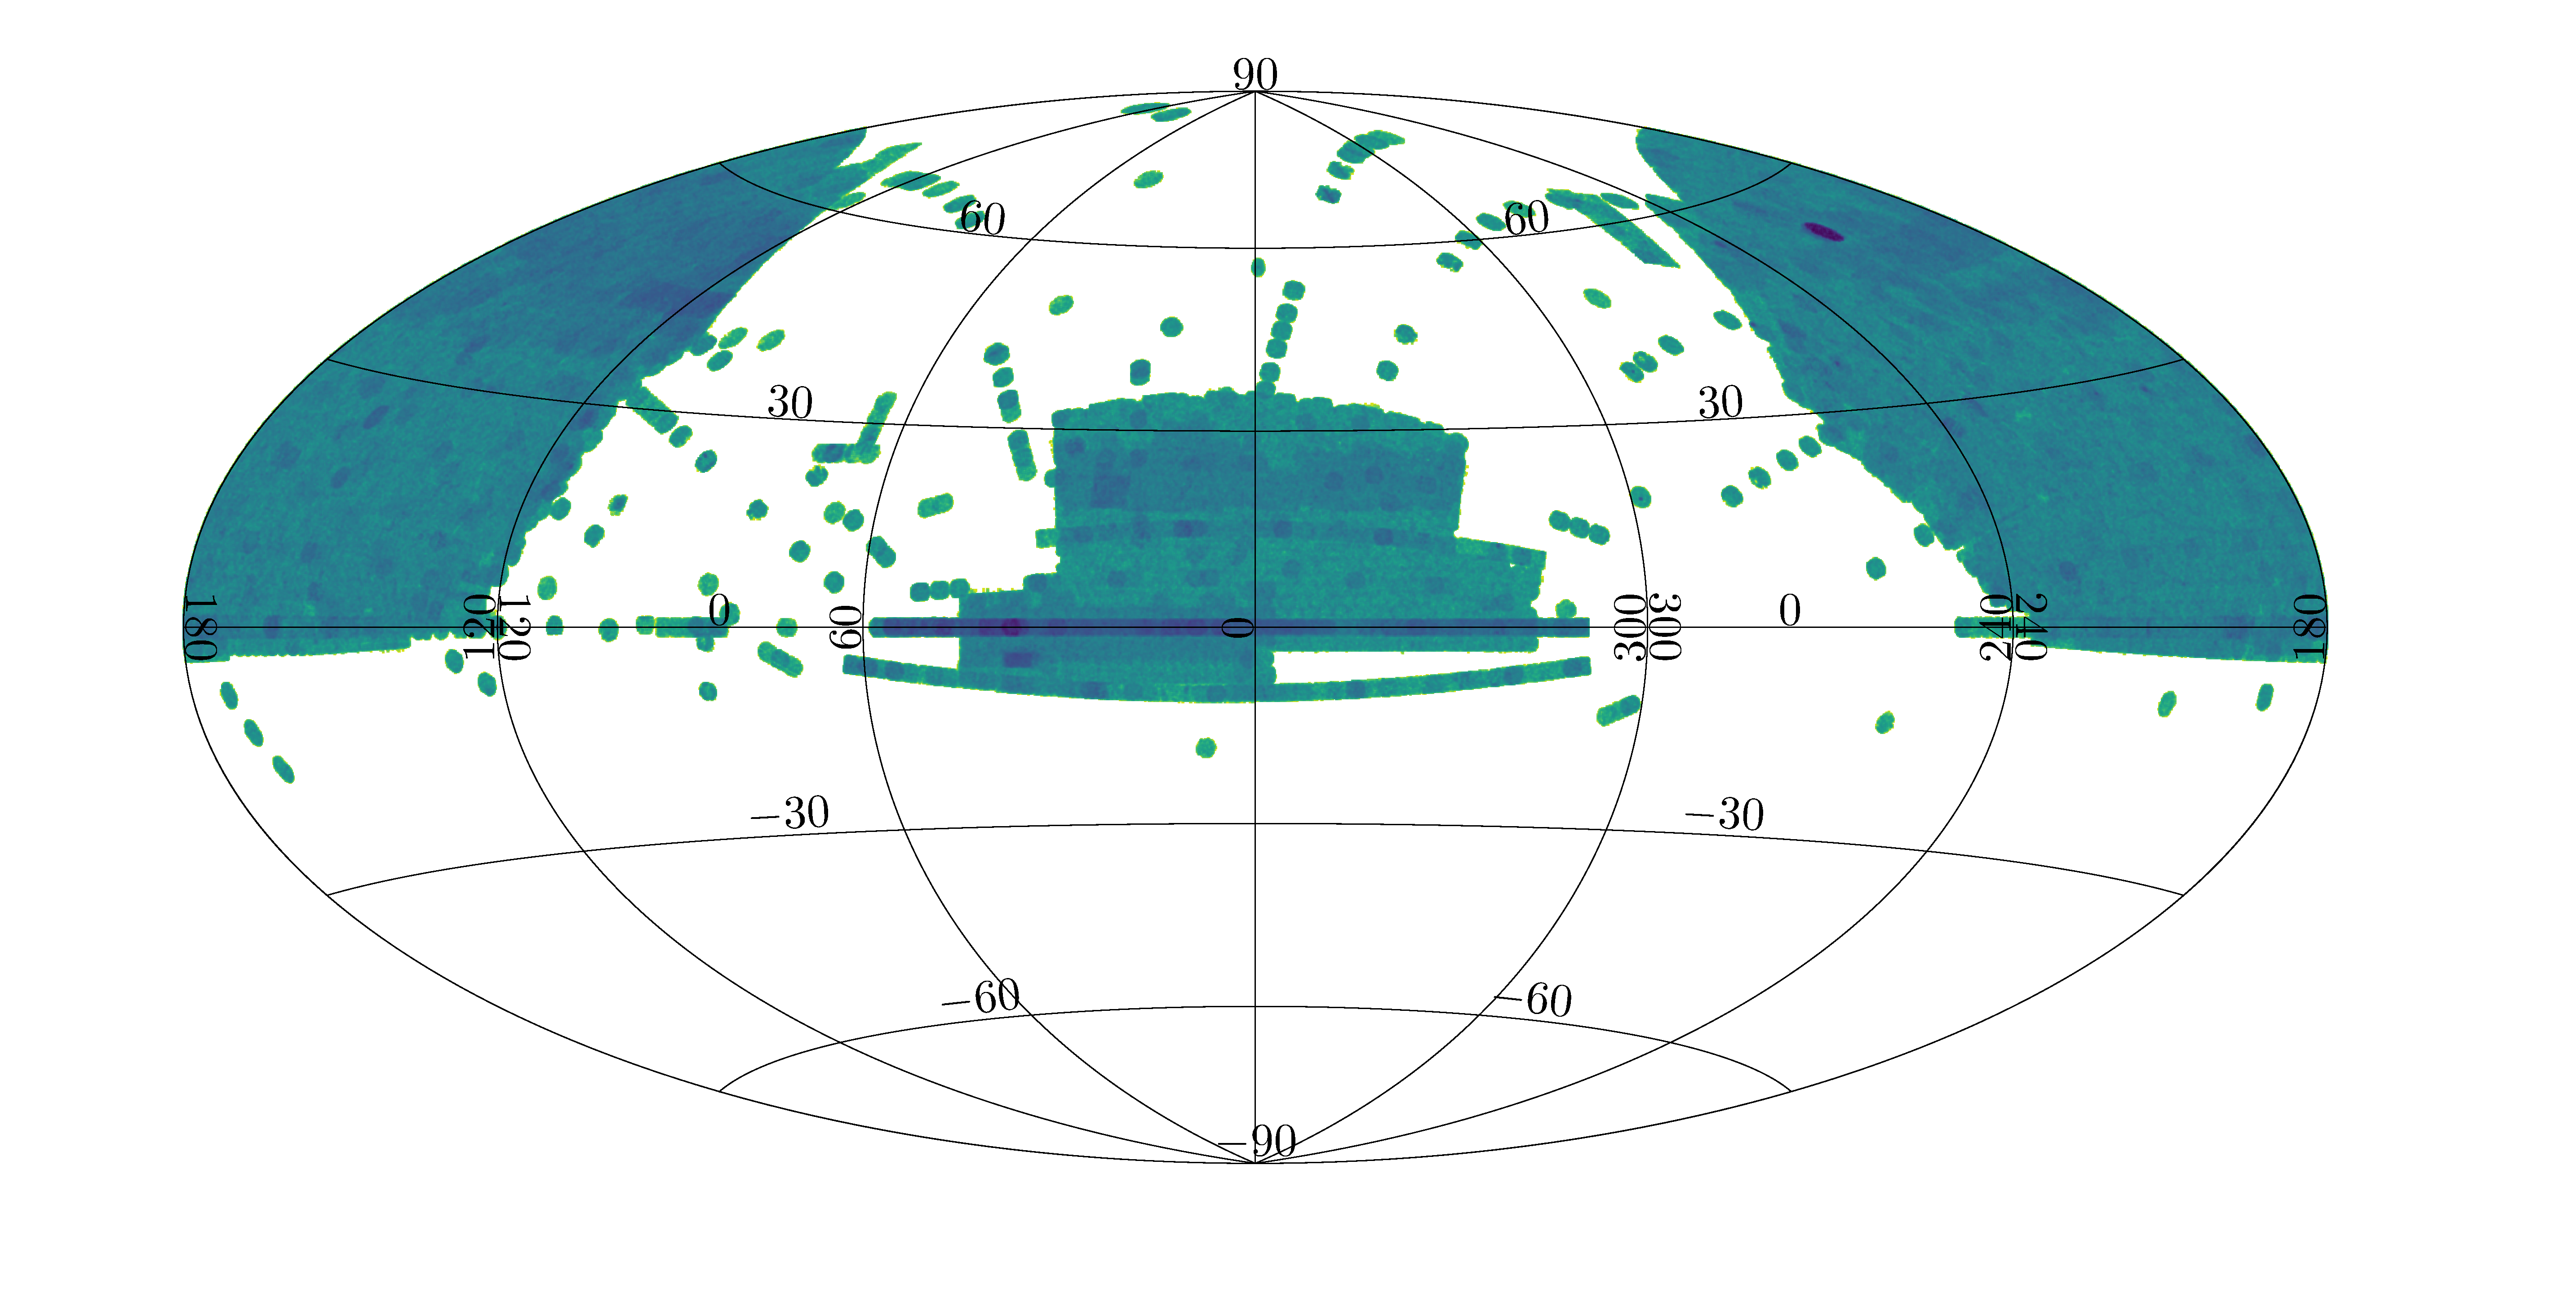
\includegraphics[width=\textwidth]{img/sdss.pdf}
}\\
\subfloat[][]{
	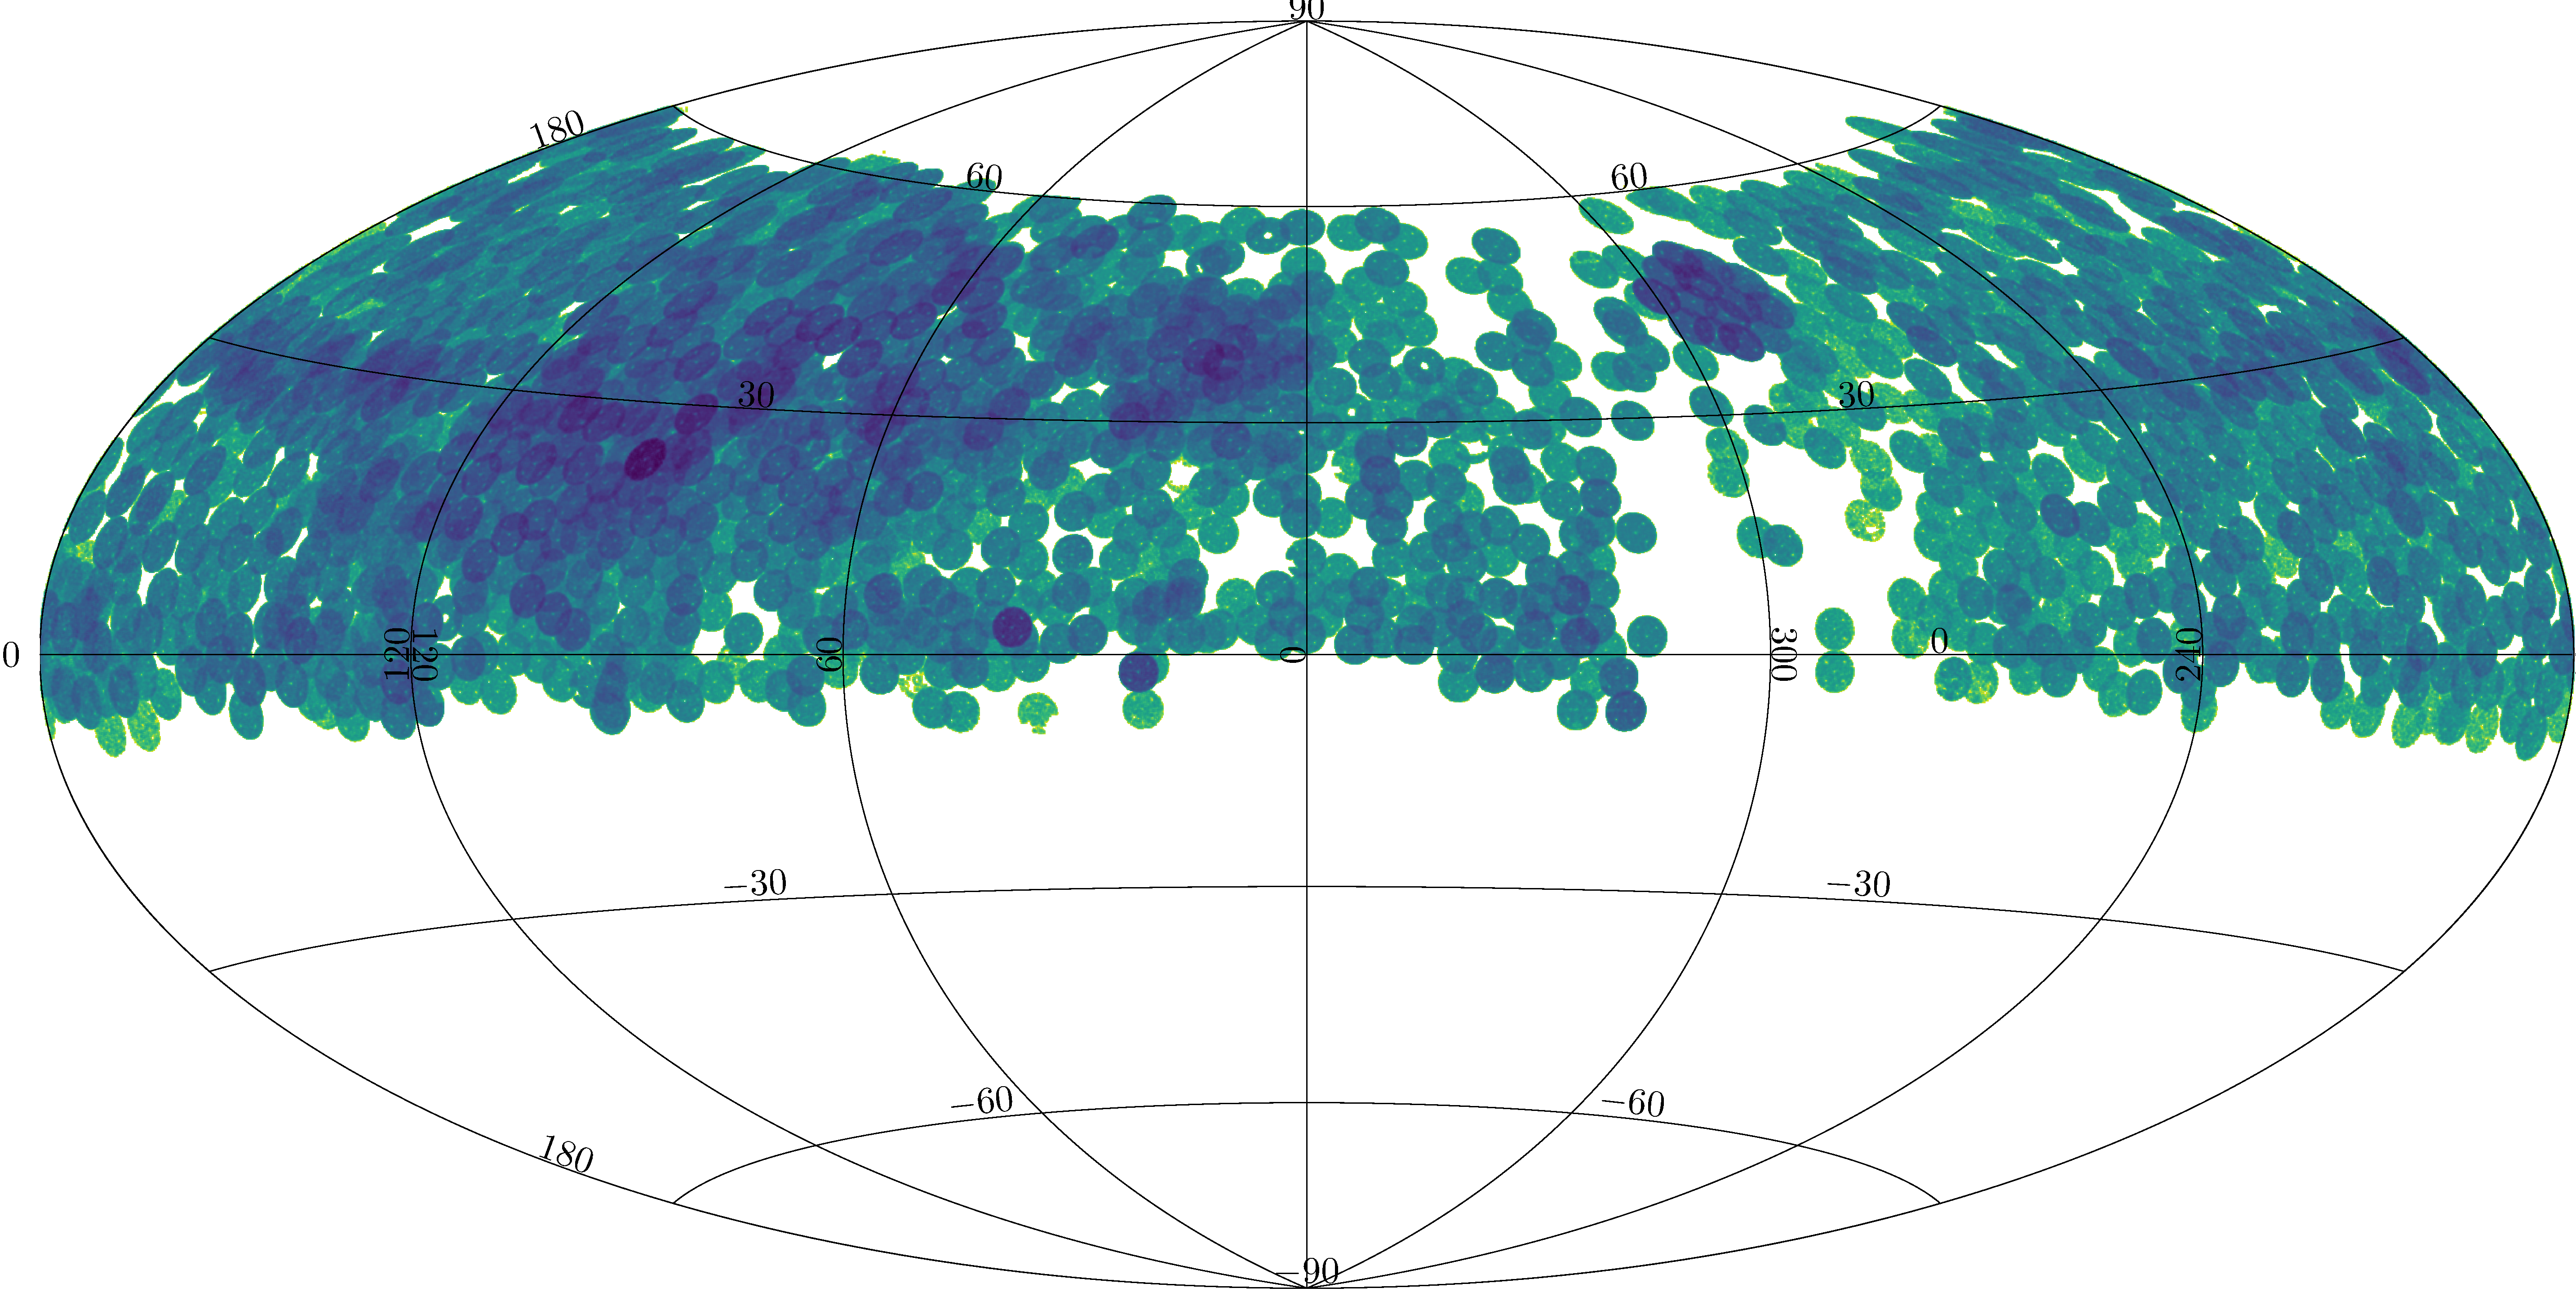
\includegraphics[width=\textwidth]{img/lamost.pdf}
}
\end{center}
\caption[Sky coverage of SDSS and LAMOST]{}
\label{sky_coverage}
\end{figure}

\begin{figure}
\begin{center}
\subfloat[][]{
	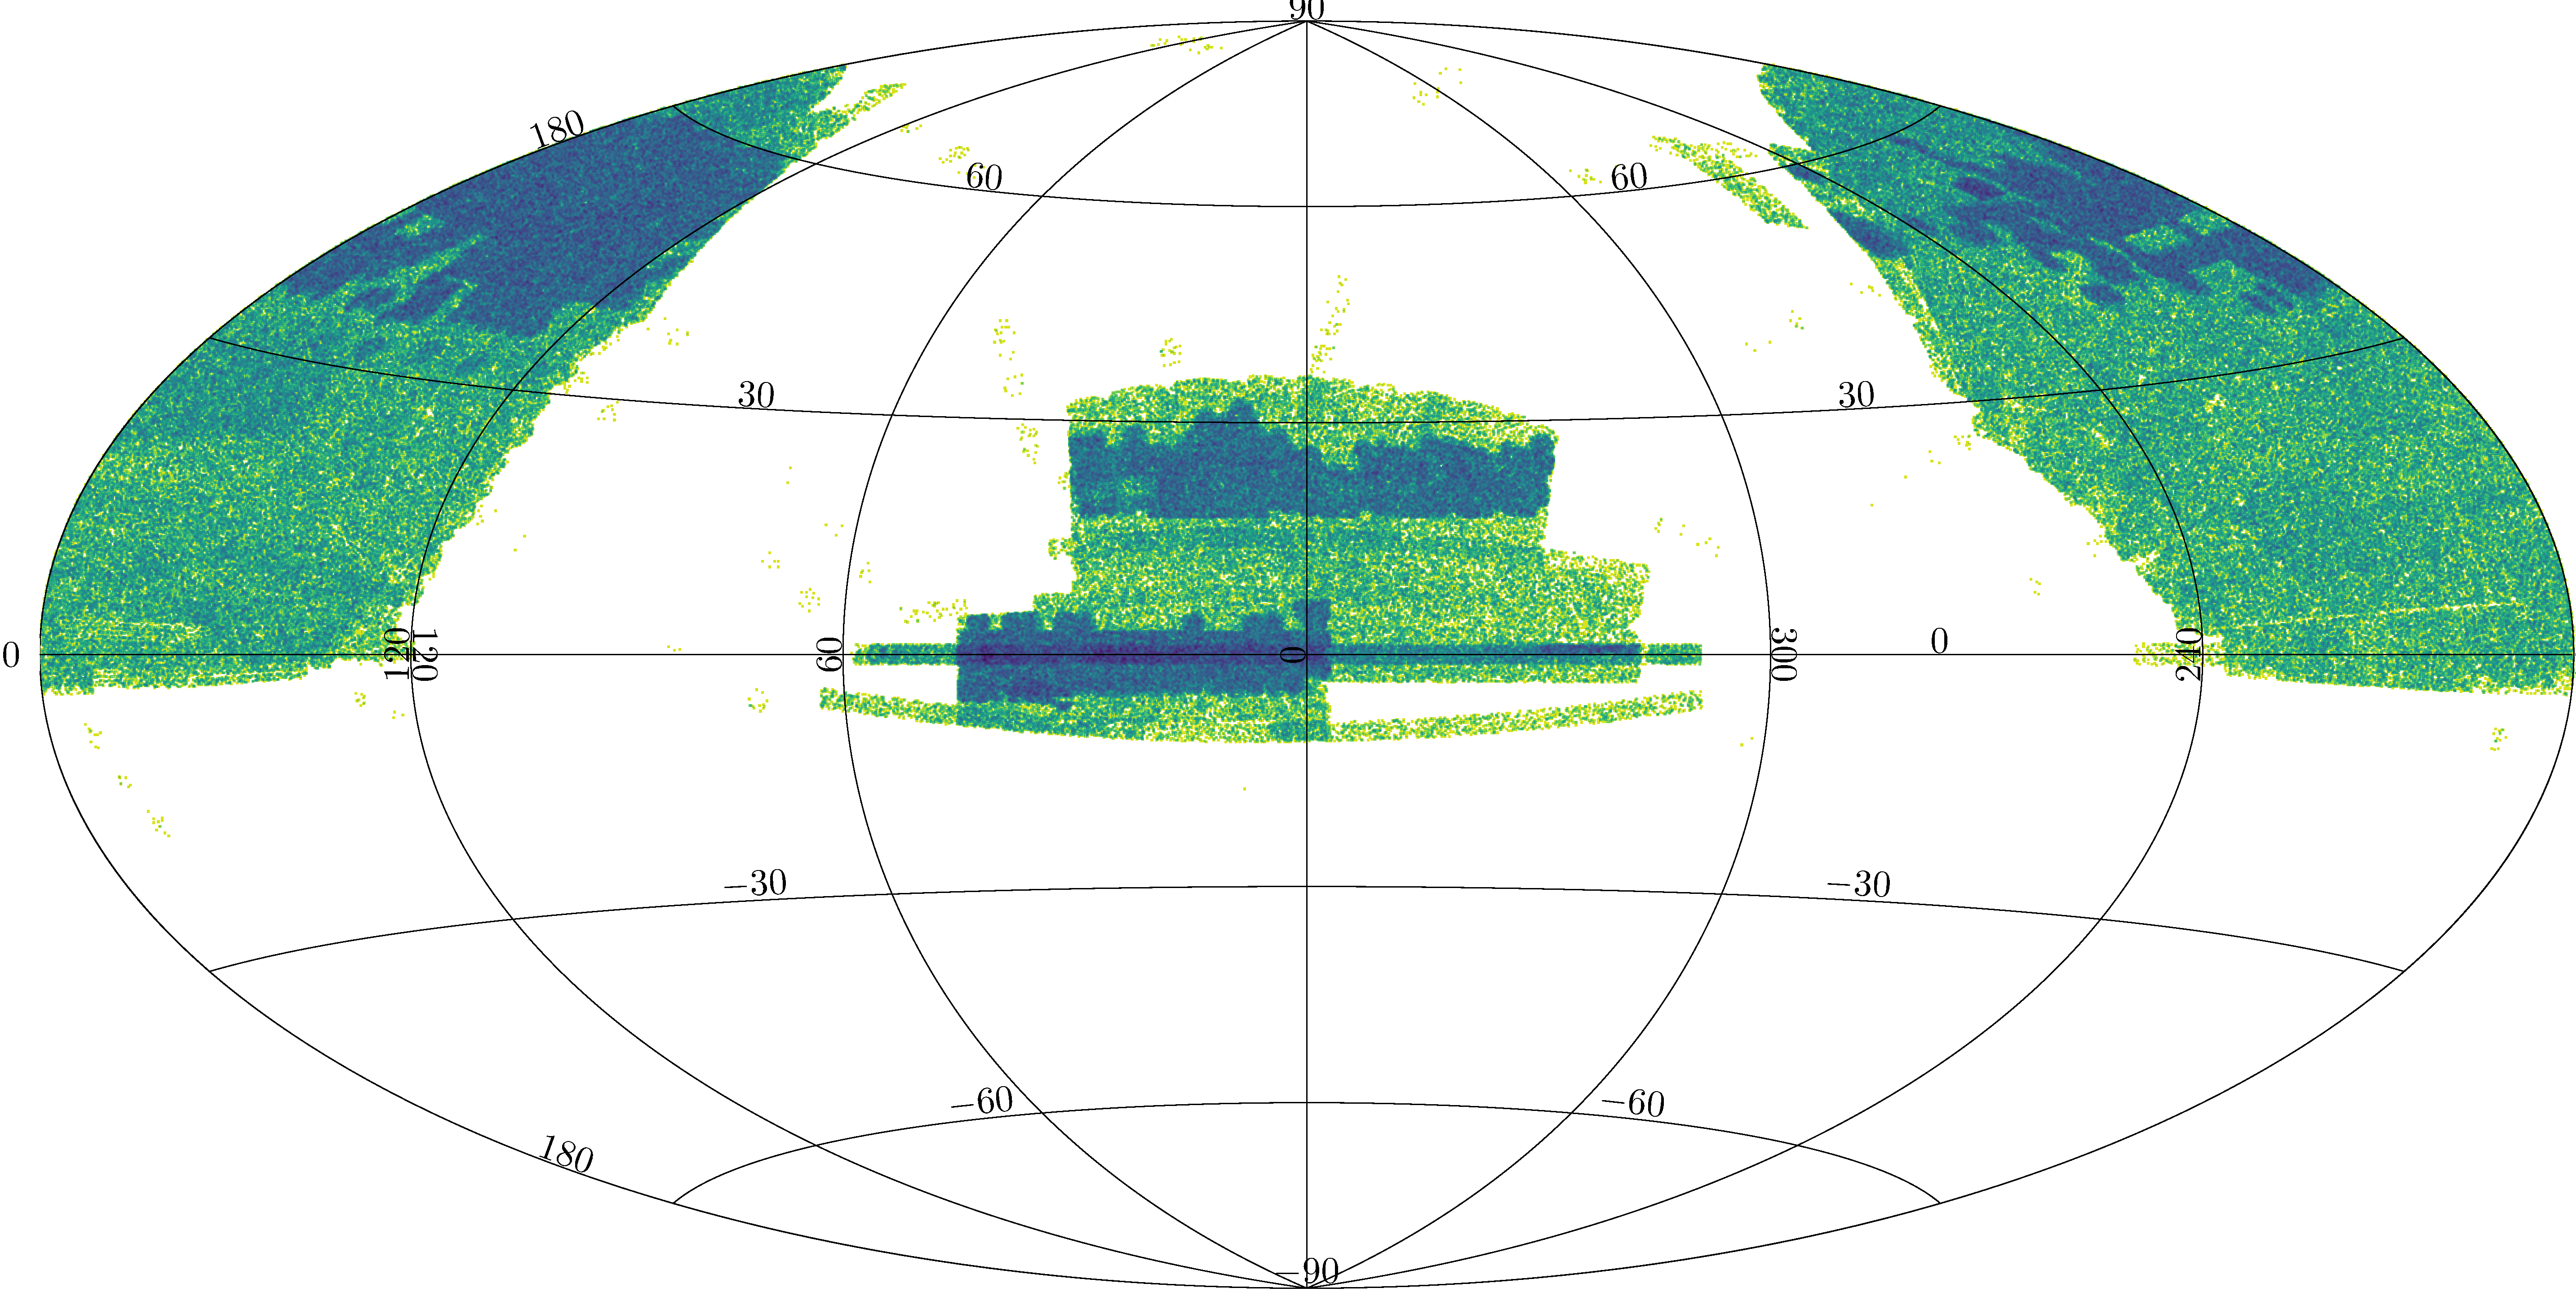
\includegraphics[width=\textwidth]{img/sdss_qsos.pdf}
}\\
\subfloat[][]{
	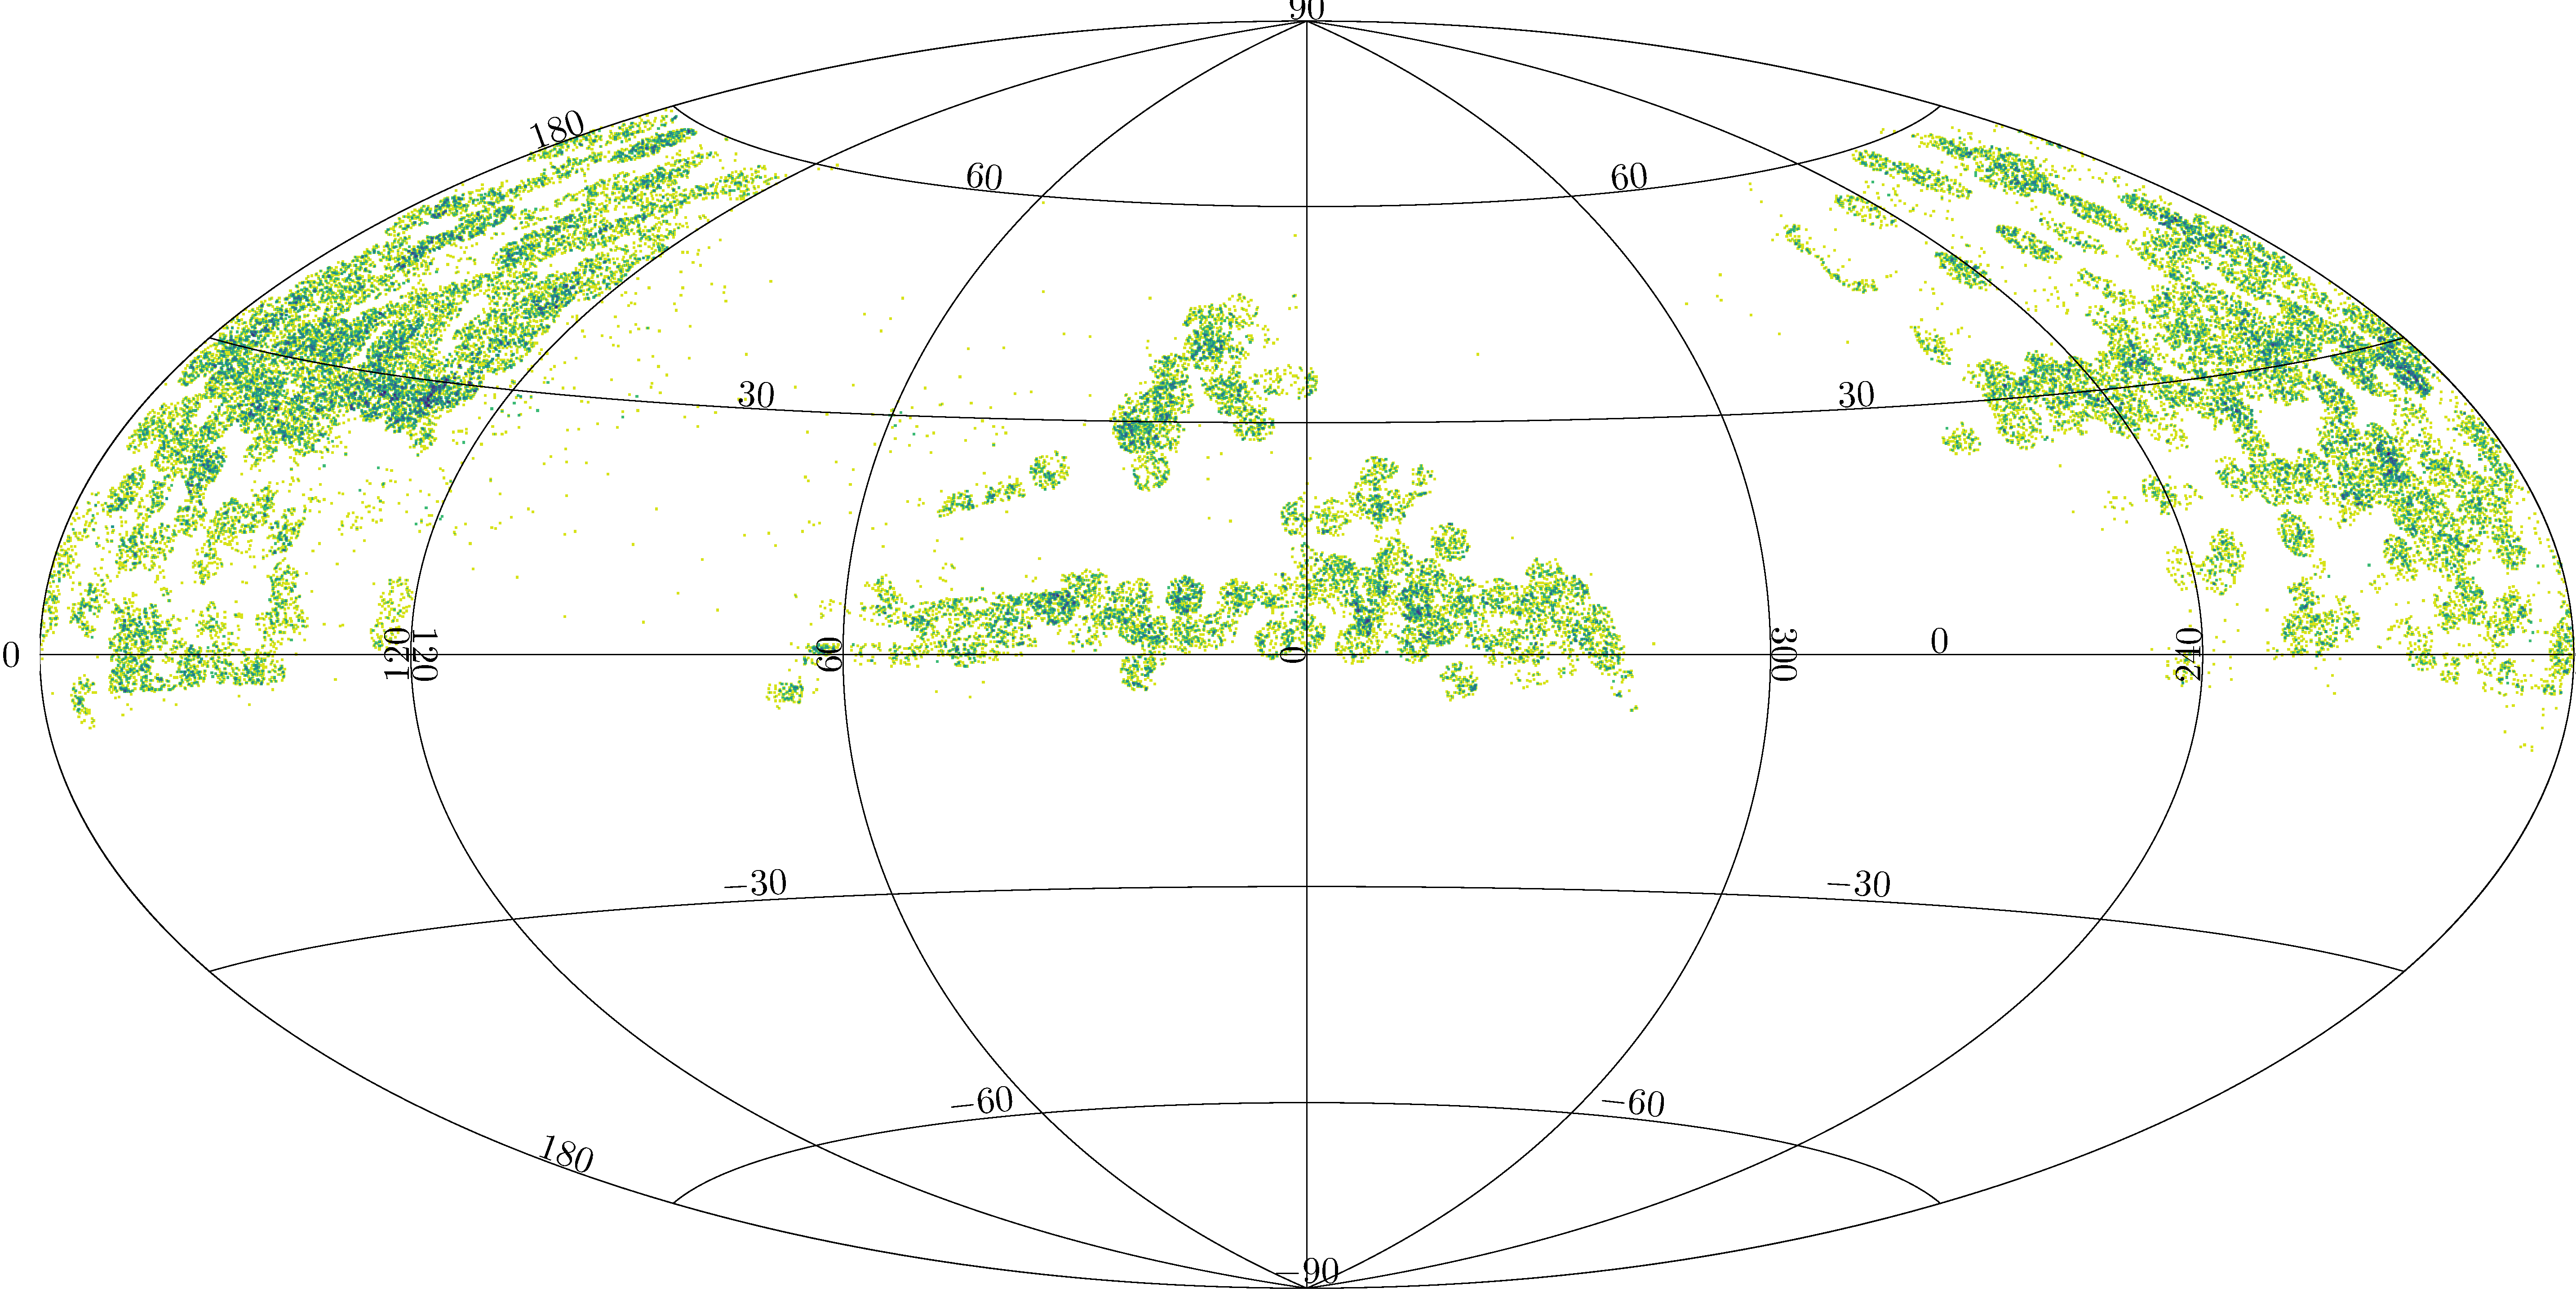
\includegraphics[width=\textwidth]{img/lamost_qsos.pdf}
}
\end{center}
\caption[QSOs coverage of SDSS and LAMOST]{}
\label{qso_coverage}
\end{figure}

We conclude that the two surveys seems to be suitable for domain adatpation
because their instrument create spectra with different resolution
and wavelegth range.
Moreover, observations of SDSS and LAMOST survey has different distribution.
